\documentclass[25pt]{tikzposter}

\usepackage{amsmath,amssymb,chemformula,graphicx,tabularx}
\usepackage[export]{adjustbox}

\geometry{paperwidth=48in,paperheight=36in,margin=0.75in}

\makeatletter
\setlength{\TP@visibletextwidth}{\textwidth-2\TP@innermargin}
\setlength{\TP@visibletextheight}{\textheight-2\TP@innermargin}
\def\TP@background{}
\makeatother

\tikzposterlatexaffectionproofoff

\usetheme{Envelope}

\hyphenpenalty=10000
\exhyphenpenalty=10000

\DeclareMathOperator{\Gal}{Gal}

\newcommand{\posterTitleStyle}[1]{{\fontsize{90}{100}\selectfont #1}}
\newcommand{\posterSubtitleStyle}[1]{{\fontsize{60}{70}\selectfont\textsc{#1}}}
\newcommand{\posterAuthorStyle}[1]{{\fontsize{48}{60}\selectfont #1}}
\newcommand{\posterInstituteStyle}[1]{{\fontsize{40}{48}\selectfont #1}}
\newcommand{\posterSectionStyle}[1]{{\fontsize{54}{60}\selectfont\bfseries #1}}
\newcommand{\posterBodyStyle}{\fontsize{40}{50}\selectfont}
\newcommand{\posterSmallStyle}{\fontsize{24}{28}\selectfont}
\newcommand{\pblock}[2]{\block{\posterSectionStyle{#1}}{\posterBodyStyle #2}}

\title{\posterTitleStyle{Molecular Symmetry and Cyclotomic Structure}}
\author{\posterSubtitleStyle{Galois Actions on Finite Symmetry Groups}\\\posterAuthorStyle{Margaret Barker, Advisor: Lilit Martirosyan}}
\institute{\posterInstituteStyle{University of North Carolina Wilmington, Department of Mathematics and Statistics}}

\begin{document}
\maketitle
\node [right=3.5cm, yshift=-6cm] at (topleft) {
\includegraphics[width=15cm]{figures/uncw_logo.png}};


\begin{columns}

    \column{0.00333}
    \column{0.33}
    \pblock{1. Molecular Symmetry\\and Point Groups}{
        A molecule's \textbf{symmetry operations} (reflections, rotations, and inversions) form a group under composition. Each molecule is classified by its \textbf{point group}, a collection of symmetry operations that leave one point fixed.\vspace{1.5em}

        \textbf{Examples:}\vspace{1em}
        
        \begin{tabular}{cccc}
            $C_{2v}$ & $C_{3v}$ & $T_d$ & $D_{6h}$\\
            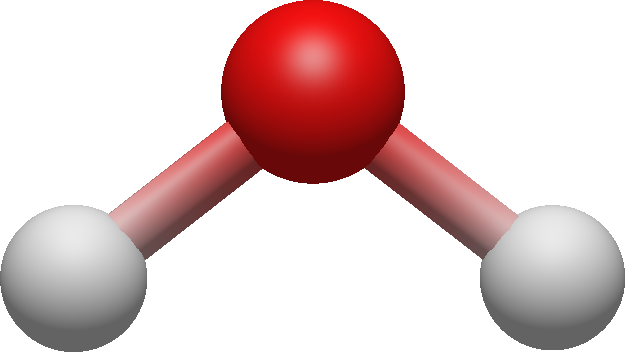
\includegraphics[width=0.24\linewidth, valign=m]{figures/c2vexample.png} & 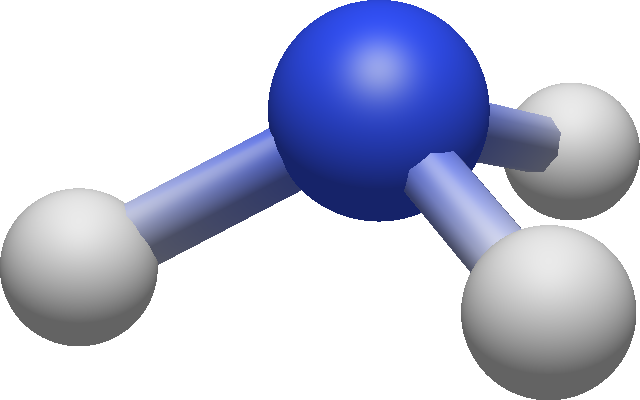
\includegraphics[width=0.24\linewidth, valign=m]{figures/c3vexample.png} & 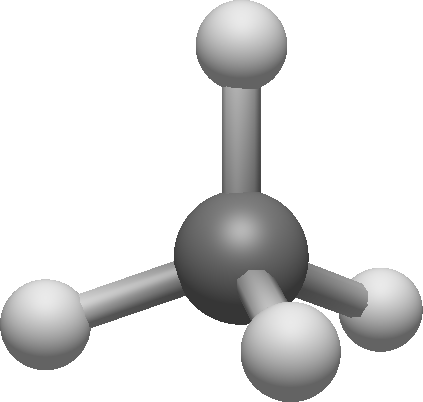
\includegraphics[width=0.24\linewidth, valign=m]{figures/tdexample.png} & 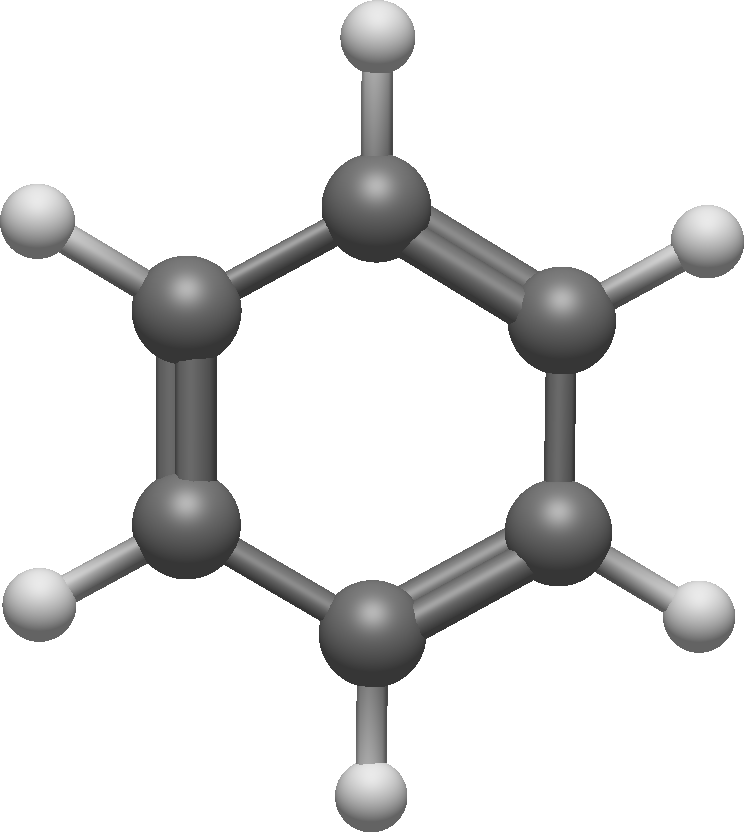
\includegraphics[width=0.24\linewidth, valign=m]{figures/d6hexample.png}\\
            water&ammonia&methane&benzene\\
            \ch{H2O}&\ch{NH3}&\ch{CH4}&\ch{C6H6}
        \end{tabular}
    }

    \pblock{2. Representations\\and Character Tables}{
        A \textbf{representation} assigns a matrix to each symmetry operation, allowing molecular symmetry to be studied with linear algebra. The \textbf{character} of an operation is the trace of its matrix. Since traces are constant on conjugacy classes, they can be organized into a \textbf{character table}, encoding the irreducible representations of the point group.\vspace{1.51em}

        \textbf{Examples:}\vspace{1em}
        
        {
            \centering
            \renewcommand{\arraystretch}{1.5}
            \begin{tabular}{c p{1.7em} c}
                \begin{tabularx}{0.5\linewidth}{>{\centering\arraybackslash}X|
                             >{\centering\arraybackslash}X
                             >{\centering\arraybackslash}X
                             >{\centering\arraybackslash}X
                             >{\centering\arraybackslash}X}
                    $C_{2v}$ & $E$ & $C_2$ & $\sigma_{v1}$ & $\sigma_{v2}$\\
                    \hline
                    $A_1$ & $1$ & $1$ & $1$ & $1$\\
                    $A_2$ & $1$ & $1$ & $-1$ & $-1$\\
                    $B_1$ & $1$ & $-1$ & $1$ & $-1$\\
                    $B_2$ & $1$ & $-1$ & $-1$ & $1$\\
                \end{tabularx}&&
                \raisebox{12mm}{
                \begin{tabularx}{0.4\linewidth}{>{\centering\arraybackslash}X|
                             >{\centering\arraybackslash}X
                             >{\centering\arraybackslash}X
                             >{\centering\arraybackslash}X}
                    $C_{3v}$ & $E$ & $2C_3$ & $3\sigma_{v}$\\
                    \hline
                    $A_1$ & $1$ & $1$ & $1$\\
                    $A_2$ & $1$ & $1$ & $-1$\\
                    $E$ & $2$ & $-1$ & $0$\\
                \end{tabularx}}
            \end{tabular}
        }
    }

    \column{0.33}
    \pblock{3. Eigenvalues\\of Symmetry Operations}{
        In a chosen representation, each symmetry operation is represented by a matrix whose eigenvalues encode its structure. If the operation has order $n$, the eigenvalues are \textbf{$n$th roots of unity}. The following diagram shows the eigenvalues of the rotation $C_3$ using the natural 3D spatial representation.\vspace{0.99em}

        \begin{center}
            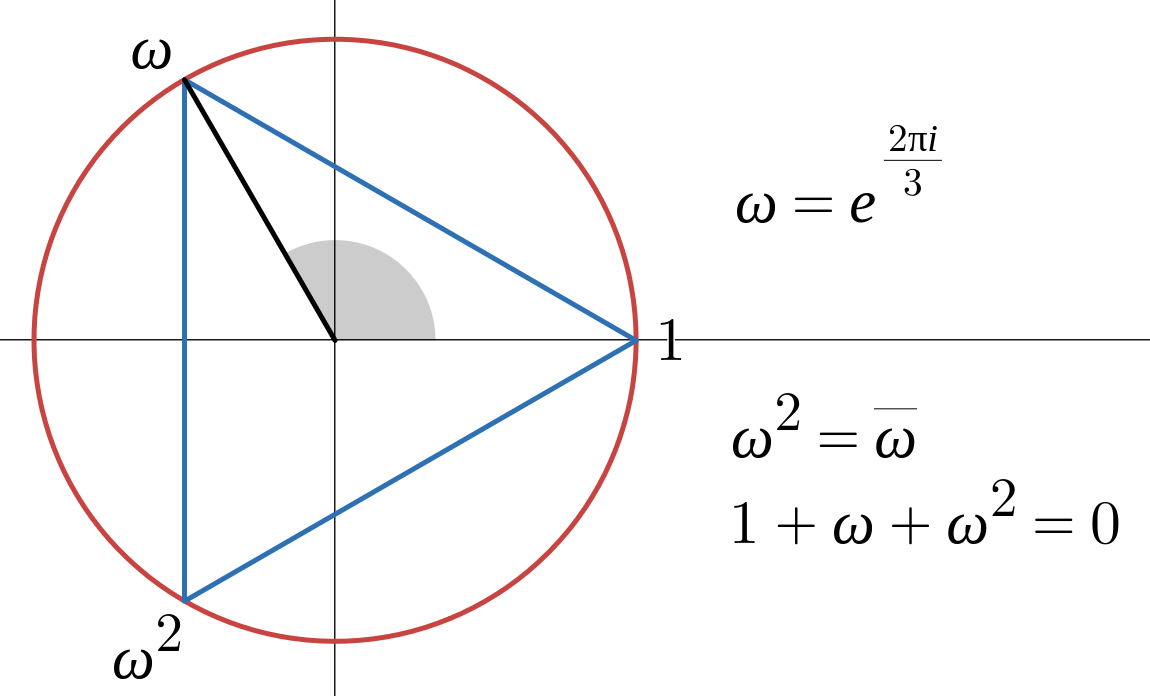
\includegraphics[width=0.55\linewidth]{figures/eigenvaluesrootsofunity.png}
        \end{center}\vspace{1em}

        The trace of a matrix is the sum of its eigenvalues. Thus, eigenvalues determine character values via the trace.
    }

    \pblock{4. Cyclotomic Structure\\of Representations}{
        Eigenvalues of symmetry operations are $n$th roots of unity, so they lie in \textbf{cyclotomic fields}. Since characters are sums of eigenvalues, they also lie in cyclotomic fields.\vspace{1em}
        
        If a symmetry operation has order $n$, its eigenvalues are powers of $\zeta_n=e^{2\pi i/n}$, and the corresponding characters lie in $\mathbb{Q}(\zeta_n)$. For $C_3$, the eigenvalues are $1,\omega,\omega^2$, so the characters lie in $\mathbb{Q}(\omega)$, where $\omega=e^{2\pi i/3}$.\vspace{1em}
        
        Mirror-plane reflections have order 2, and their eigenvalues are $\pm1$. Hence, the corresponding characters are integers.\vspace{1em}

        However, even when characters lie in $\mathbb{Q}(\zeta_n)$, they may still be integers. For example, in the point group $C_{3v}$, all of the characters are integers, despite the presence of $C_3$ rotations. This observation leads to a connection between characters and Galois theory. 
    }

    \column{0.33}
    \pblock{5. Galois Actions\\on Character Values}{
        Cyclotomic fields $\mathbb{Q}(\zeta_n)$ have symmetries given by \textbf{Galois automorphisms}, which form the group \[G=\Gal(\mathbb{Q}(\zeta_n)/\mathbb{Q})\cong(\mathbb{Z}/n\mathbb{Z})^\times.\] For $1\le k<n$ with $\gcd(k,n)=1$, there exists $\sigma_k\in G$ such that $\sigma_k(\zeta_n)=\zeta_n^k$. These automorphisms permute eigenvalues of matrices whose characteristic polynomials lie in $\mathbb{Q}[x]$.\vspace{1.31em}

        The irreducible representation $E$ of $C_{3v}$ corresponds to matrix blocks with characteristic polynomials in $\mathbb{Q}[x]$. Hence, $G$ permutes their eigenvalues. In this case, character values are fixed under $G$, hence rational. Also, character values are algebraic integers, and the only rational algebraic integers are ordinary integers. Thus, the character values of $C_{3v}$ are integers. For example, for the $C_3$ rotation, $G$ permutes the eigenvalues, $\omega, \omega^2$, while fixing their sum, $\omega+\omega^2=-1$.
    }

    \pblock{6. Fivefold Symmetry\\and Non-Integer Characters}{
        For fivefold symmetry, the eigenvalues are $1,\xi,\xi^2,\xi^3,\xi^4$, where $\xi=e^{2\pi i/5}$. Galois automorphisms permute these eigenvalues, but sums like $\xi\,+\,\xi^4=2\cos(2\pi/5)\in\mathbb{Q}(\sqrt{5})$ are not rational. As a result, in point groups such as $C_{5v}$ or $D_{5d}$, some characters lie in $\mathbb{Q}(\sqrt5)$, not $\mathbb{Z}$.\vspace{1.05em}

        \textbf{Examples:}\vspace{1em}
        
        \begin{tabular}{c p{0.5em} c}
            $C_{5v}$ & & $D_{5d}$\\
            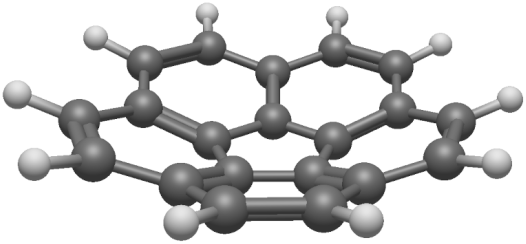
\includegraphics[width=0.6\linewidth, valign=m]{figures/corannulenesmall.png} & &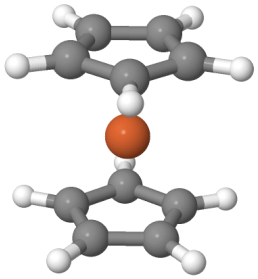
\includegraphics[width=0.24\linewidth, valign=m]{figures/ferrocenesmall.png}\\
            corannulene& &ferrocene (staggered)\\
            \ch{C20H10}& &\ch{Fe(C5H5)2}
        \end{tabular}
    }
\end{columns}

\end{document}